\documentclass{article} % For LaTeX2e
\usepackage{nips13submit_e,times}
\usepackage{hyperref}
\usepackage{url}
\usepackage{graphicx}
\usepackage{amssymb}


\title{Popularity of content leads to its duplication on Reddit}

% The \author macro works with any number of authors. There are two commands
% used to separate the names and addresses of multiple authors: \And and \AND.
%
% Using \And between authors leaves it to \LaTeX{} to determine where to break
% the lines. Using \AND forces a linebreak at that point. So, if \LaTeX{}
% puts 3 of 4 authors names on the first line, and the last on the second
% line, try using \AND instead of \And before the third author name.

\newcommand{\fix}{\marginpar{FIX}}
\newcommand{\new}{\marginpar{NEW}}

\nipsfinalcopy % Uncomment for camera-ready version

\begin{document}

\maketitle

\begin{abstract}
On social network sites like Reddit, users submit links or share textual content. The community upvotes (for) and downvotes (against) and reddit uses community sourcing as a means to order content. The contributed are scored that is number of upvotes minus downvotes. The popularity of a user is represented by his/her karma. In this project, we have tried to judge how the popularity of contents leads to its duplication on Reddit. Users can re-post the popular posts on various other subreddits in order to receive more upvotes, and thus increasing their karma. The results from this project will depict  how the users satisfy their Reddit Karma and the design implications of this in online communities.
\end{abstract}

\section{Objectives}
We will be mainly focusing on the following in our project to depict how the users satisfy their Reddit Karma and the design implications of this in online communities. We will correlate a post's score with its diffusion into other subreddits. We will also try to find the existence of a user type where most of the users' posts are reposts and fresh content contribution by this user type is less. Finally, we will correlate increase in link karma with the number of reposts of a user.

\section{Background Study}

As social networks and the user-generated content that populates them continue to grow in prevalence, size, and influence, understanding how users interact and produce this content becomes increasingly important. Insight into these community dynamics could prove valuable for measuring content trust, providing role-based group recommendations, or evaluating group stability and growth. For the related work, we have done readings of three papers, namely, Eric Gilbert's - ``Widespread Under Provision on reddit'', Cody Buntain's - ``Identifying social roles in reddit using network structure'' and Donn Morrison's - ``Here, have an upvote: communication behaviour and karma on Reddit''.

Online communities rely on their members to do work for the good of everyone on the site. The links with the most up-votes bubble up to the main page, pointing everyone toward the best content. However, when too many people rely on others to contribute without doing so themselves results in underprovision. Gilbert observed that Reddit overlooked 52\% of the most popular links the first time they were submitted [1]. This suggests that many potentially popular links get ignored, thus jeopardizing the site's core purpose of showing the best voted content. 

Cody Buntain has identified well-known behavioral patterns and social roles in the multi-community environments. In his paper, he has demonstrated the presence and identifiability of the answer-person role in reddit and showed that only a very small number of users participate across community boundaries [2]. 
				
Donn Morrison has tried to cluster the users of Reddit.com into behavioural roles using features derived from their egocentric reply-graphs. He has tried to explore the link between the distribution of karma (i.e. popularity measured by the number of up- and downvotes) and the behavioural role to which that user belongs. He observed that users with Contributor behaviour proved to be more popular, however the variance in karma in this role was high [3]. Thus, this indicates that the contributor role encompasses both popular and unpopular users. By predicting high-karma users, community owners or moderators, or even the users themselves, could more efficiently manage and maintain behaviour in the forums such as Reddit.com under analysis.	

All three papers have tried to examine the users and the data posted by them on Reddit.com. They demonstrated that most of the popular links are overlooked in the first time, only a small number of users participate across community boundaries and the behavioural role of the user is directly linked to the distribution of karma. 

In this project, we are also trying to examine the users and their activity. We are trying to demonstrate that popularity of content leads to its duplication on Reddit. In order to achieve this, we have used the Reddit API to collect the data across various subreddits at various times of the day. 


\section{Data Collection}

\subsection{Identification of Subreddits}

So far, We chose subreddits related to photography. This was done as all reddit posts on such subreddits use image sharing services like imgur.com. These sharing services usually generate an unique url for each gallery that can be used to share on reddit. Hence, by searching for posts with same image urls, we were able to identify duplicate posts.

Reddit has an inbuilt subreddit recommendation system which lists down relevant subreddits for every search query. These subreddits have a varying frequency of user posts, thus giving a uniform result instead of results being biased to only few with the maximum activity. We choose 10 subreddits to get a preliminary idea about the posts and users in a subreddit.

The subreddits chosen for this study were: 

\begin{itemize}
\item /pics
\item /gifs
\item /picrequests
\item /photography
\item /Images
\item /itookapicture
\item /postprocessing
\item /photocritique
\item /HDR
\item /shittyHDR
\end{itemize}

For the project rest of the semester, we plan to re-choose subreddits after a meeting with the professor. Since search allows us to search throughout reddit, we don't have to pick subreddits close to each other. 

\subsection{Fetching and Storing}

We then used Reddit API to retrieve the content (link submissions on hot page) from these subreddits by using an API wrapper (PRAW - python reddit api wrapper) provided for Python language. The script was executed for one hour each on four different times in the same day, to add the dimension of time in our content analysis. A MySQL database was used to store and update the tables of the content which was fetched. While data collection of top and news posts is running, in parallel, we also run a bot that looks at posts that has been collected more than 5 days in the past and we look up where have these links diffused in reddit and stores the tuple (link, sub\_reddit, poster, time\_created) into the db. 

\section{Data Analysis}

The statistics of the data collected can be seen in Table1.

\begin{table}
\begin{center}
    \begin{tabular}{ | l | l | }
    \hline
    Number of Posts & 42992 \\ \hline
    Number of Unique Authors & 33044 \\ \hline
    Number of links reposted at least once & 7541 \\ \hline
    \end{tabular}
    \caption{Contributions}
\end{center}
\end{table}

\subsection{Chains}

Once we have obtained all the posts, we search each of the posts on reddit in order to get their diffusion across the various sub-reddits since their inception. Thus, we thinking of the search results like a diffusion chain. We have sorted the results by time and we call the first person to post the link as the original author. How many times the original author posts initially is how much effort he puts into broadcasting the link. After this, we have found the search result with max score so that we can know when a particular reached its maximum popularity. All results to the left of the max post form the left chain and after wards form the right chain.

An example of chains can be seen in the following figure:

\begin{figure}[h]
\begin{center}
%\framebox[4.0in]{$\;$}
%\fbox{\rule[-.5cm]{0cm}{4cm} \rule[-.5cm]{4cm}{0cm}}
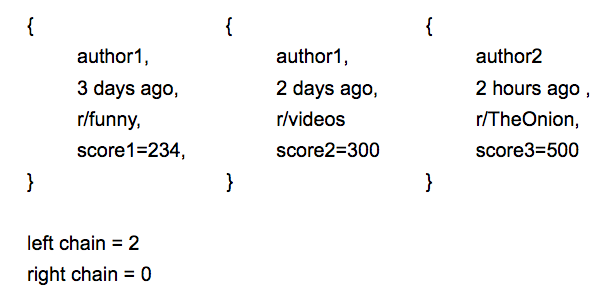
\includegraphics[width=4in]{chain.png}
\caption{Description of Chain}
\end{center}
\end{figure}

In this example, we have three results, the last result has the max score, so our left chain length is 2 and right chain length is 0.  Note that we don?t do normalization with respect to how many subscribers are in the subreddit.

\subsection{Distribution of Chain Length}

\begin{figure}[h]
\begin{center}
%\framebox[4.0in]{$\;$}
%\fbox{\rule[-.5cm]{0cm}{4cm} \rule[-.5cm]{4cm}{0cm}}
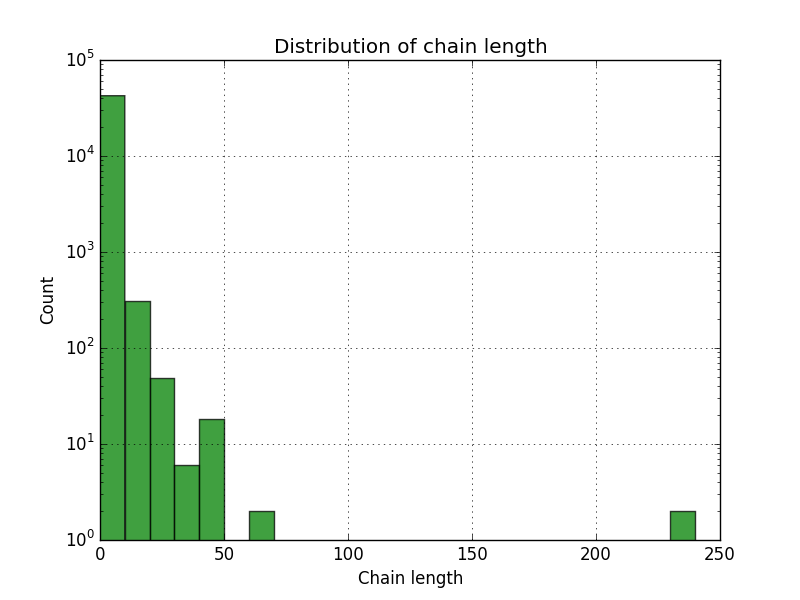
\includegraphics[width=4in]{lengths.png}
\caption{Distribution of Chain Length}
\end{center}
\end{figure}


\subsection{Distribution of Original Author Re-posting}

\begin{figure}[h]
\begin{center}
%\framebox[4.0in]{$\;$}
%\fbox{\rule[-.5cm]{0cm}{4cm} \rule[-.5cm]{4cm}{0cm}}
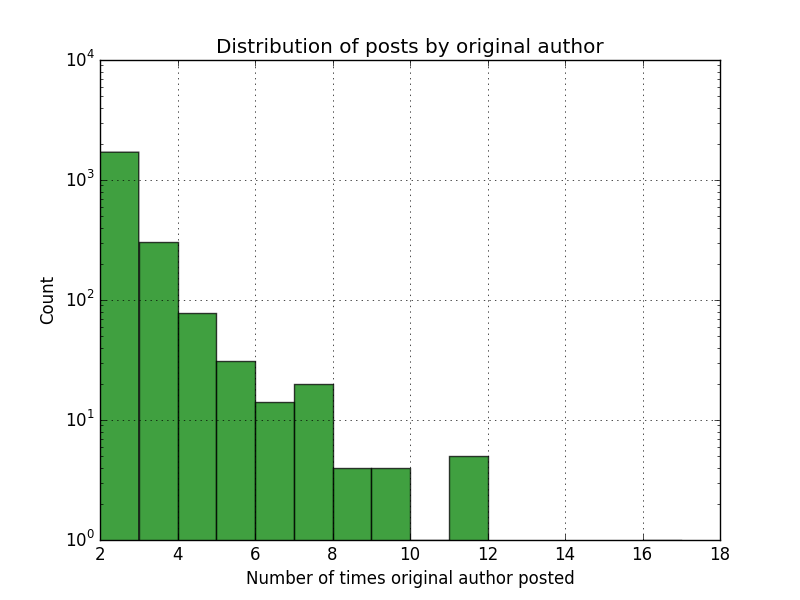
\includegraphics[width=4in]{original_author.png}
\caption{Distribution of Original Author Re-posting}
\end{center}
\end{figure}


\subsection{Distribution of Re-posts by each Subreddit}

\begin{figure}[h]
\begin{center}
%\framebox[4.0in]{$\;$}
%\fbox{\rule[-.5cm]{0cm}{4cm} \rule[-.5cm]{4cm}{0cm}}
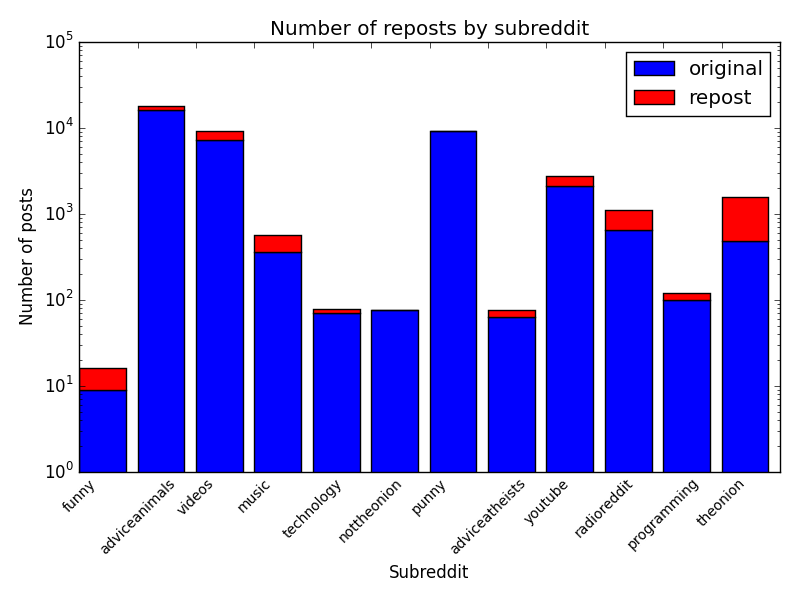
\includegraphics[width=4in]{reposts.png}
\caption{Distribution of Re-posts by each Subreddit}
\end{center}
\end{figure}


\subsection{Distribution of Different Authors Re-posting}

\begin{figure}[h]
\begin{center}
%\framebox[4.0in]{$\;$}
%\fbox{\rule[-.5cm]{0cm}{4cm} \rule[-.5cm]{4cm}{0cm}}
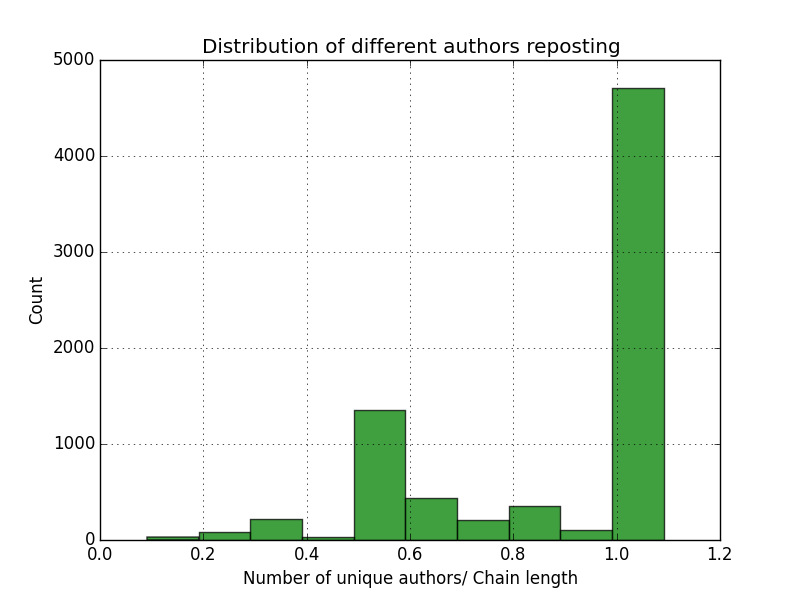
\includegraphics[width=4in]{unique_authors.png}
\caption{Distribution of Different Authors Re-posting}
\end{center}
\end{figure}

\subsection{Distribution of Left Chain Length}

\begin{figure}[h]
\begin{center}
%\framebox[4.0in]{$\;$}
%\fbox{\rule[-.5cm]{0cm}{4cm} \rule[-.5cm]{4cm}{0cm}}
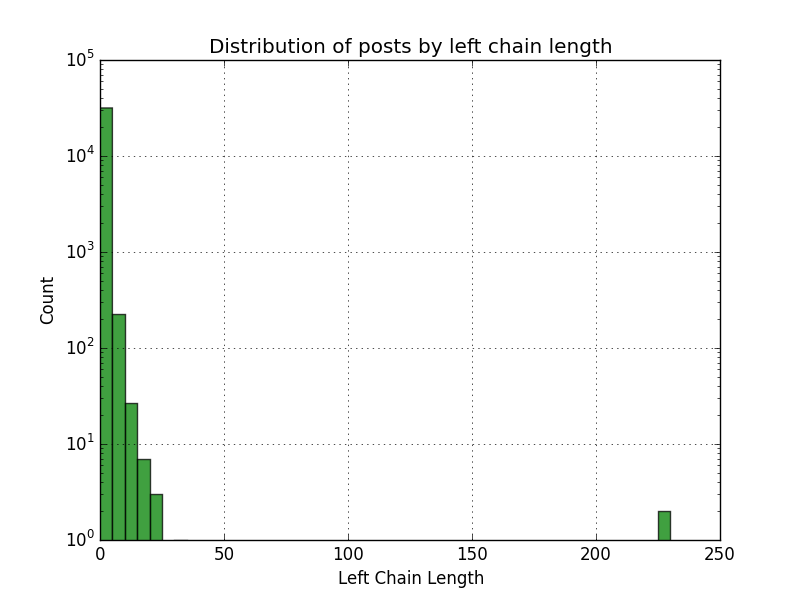
\includegraphics[width=4in]{left_chain.png}
\caption{Distribution of Left Chain Length}
\end{center}
\end{figure}

\subsection{Distribution of Right Chain Length}

\begin{figure}[h]
\begin{center}
%\framebox[4.0in]{$\;$}
%\fbox{\rule[-.5cm]{0cm}{4cm} \rule[-.5cm]{4cm}{0cm}}
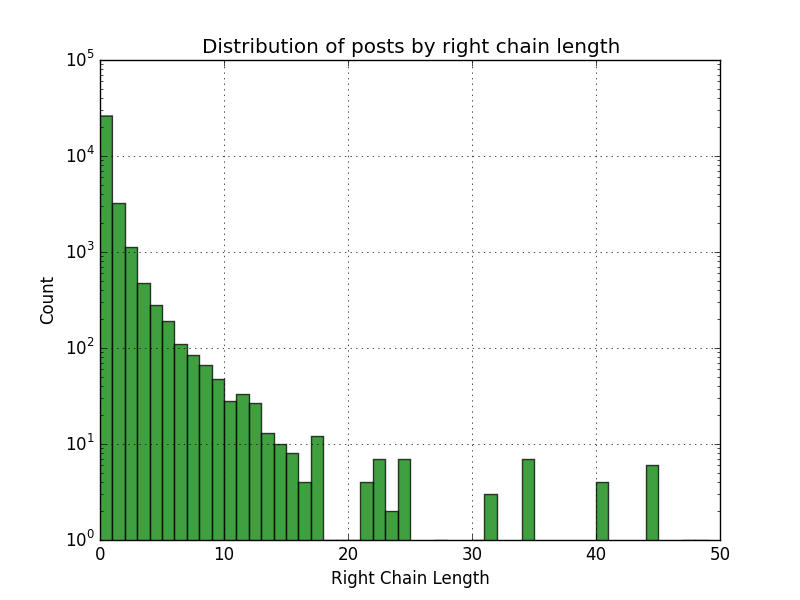
\includegraphics[width=4in]{right_chain.png}
\caption{Distribution of Right Chain Length}
\end{center}
\end{figure}

\subsection{Distribution of Max Score by the Right Chain Length}

\begin{figure}[h]
\begin{center}
%\framebox[4.0in]{$\;$}
%\fbox{\rule[-.5cm]{0cm}{4cm} \rule[-.5cm]{4cm}{0cm}}
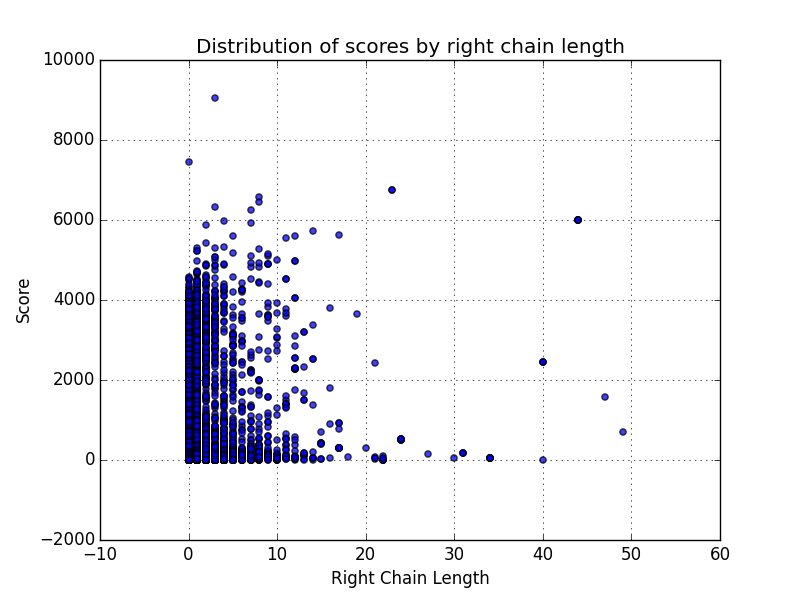
\includegraphics[width=4in]{score_right_chain.png}
\caption{Distribution of Max Score by the Right Chain Length}
\end{center}
\end{figure}

\subsection{Distribution of Maximum Score of the chains}

\begin{figure}[h]
\begin{center}
%\framebox[4.0in]{$\;$}
%\fbox{\rule[-.5cm]{0cm}{4cm} \rule[-.5cm]{4cm}{0cm}}
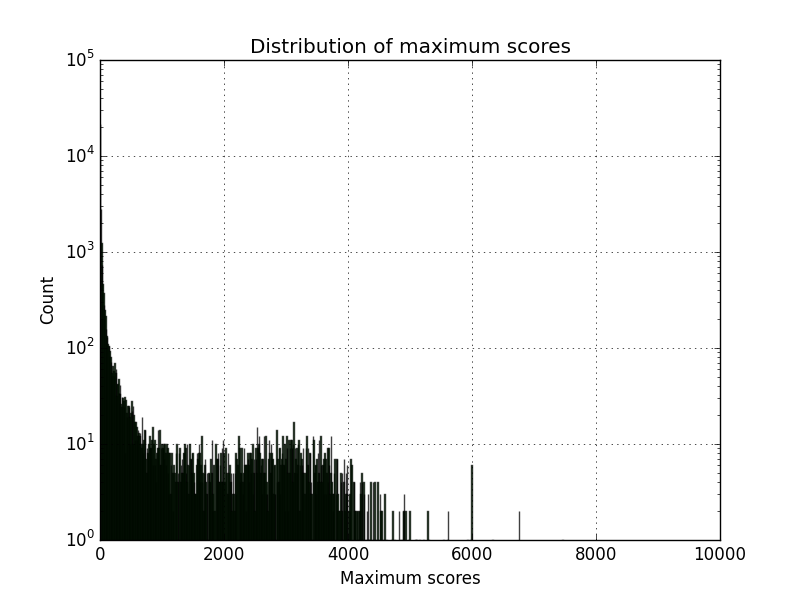
\includegraphics[width=4in]{max_score_distribution.png}
\caption{Distribution of Maximum Score of the chains}
\end{center}
\end{figure}

From the data we have collected, we have done some basic analysis and made some visualizations.

We wanted to look at the trend of how often do users contribute. Our hypothesis was the very very few users contribute worth content. Figure 1 refers to the graph between number of users and number of posts. As you can see very few users have good amount of posts. On the x-axis, it shows the counts of the posts, and on the y-axis, the corresponding number of users who have made that many posts. In the collection, we noticed that 633 users had posted single time, and this number decreased drastically as the count got number of posts increased. Figure 2 refers to the graph of number of submissions per subreddits. Figure 3 refers to the graph of mean link karma of users who have posted. Figure 4 refers to the means scores of submissions. Figure 5 refers to the number of search results and score of submission.

\section{Comparison with Eric Gilbert's Paper on Under-provision on Reddit}

\begin{figure}[h]
\begin{center}
%\framebox[4.0in]{$\;$}
%\fbox{\rule[-.5cm]{0cm}{4cm} \rule[-.5cm]{4cm}{0cm}}
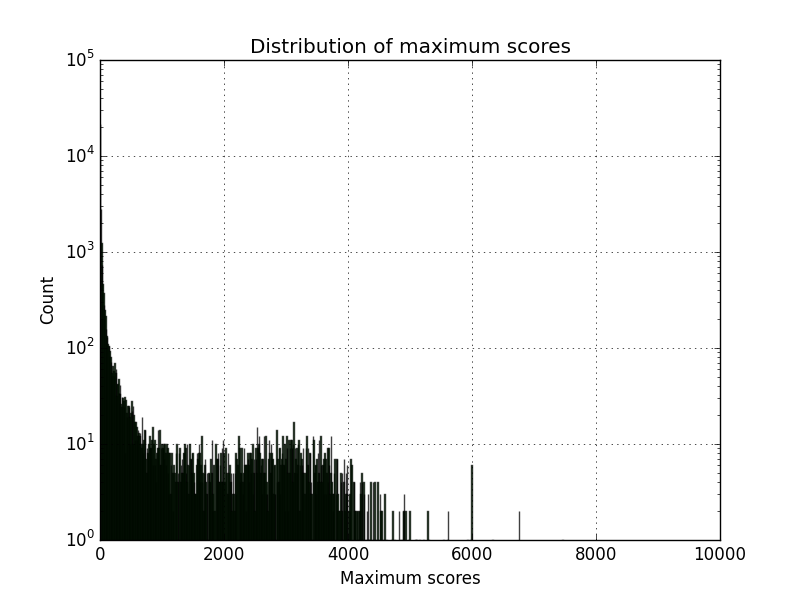
\includegraphics[width=4in]{max_score_distribution.png}
\caption{Distribution of Maximum Score of the chains}
\end{center}
\end{figure}

\begin{figure}[h]
\begin{center}
%\framebox[4.0in]{$\;$}
%\fbox{\rule[-.5cm]{0cm}{4cm} \rule[-.5cm]{4cm}{0cm}}
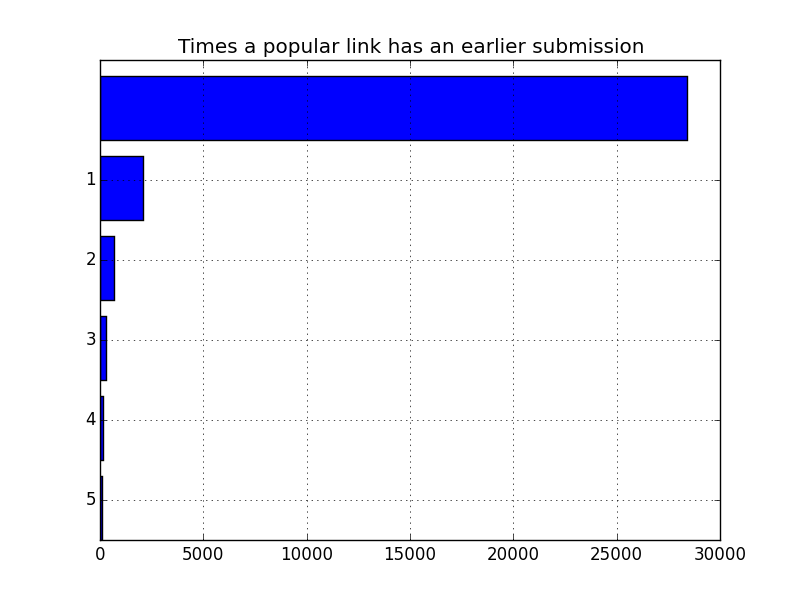
\includegraphics[width=4in]{count.png}
\caption{Times a popular link has an earlier submission}
\end{center}
\end{figure}

\section{Anomalies with the Data}

\subsection{Forbidden Links}

\subsection{Posts having chain length of 235}

\subsection{Exception Handling}

\subsection{Issue with PRAW}

\section{Future Work}

\section{Work Ahead}
For the second part of the term, we plan to collect data for 15 days from subreddits in different areas of interest and of smaller size with the new and top queue. We are planning to look at the following subreddits as shown in Table 1:

\begin{table}
\begin{center}
    \begin{tabular}{ | l | l | }
    \hline
    Famous Subreddits & Similar smaller subreddits \\ \hline
    funny (6,988,603) & punny (54,491) \\ \hline
    AdviceAnimals (4,252,660) & AdviceAtheists (13,460) \\ \hline
    videos (6,192,963) & YouTube (21,611) \\ \hline
    Music (5,526,808) & RadioReddit (13,356) \\ \hline
    technology (5,066,423) & programming (559,631) \\ \hline
    nottheonion (1,435,635) & TheOnion (6,610) \\ 
    \hline
    \end{tabular}
    \caption{Subreddits we plan to monitor and number of subscribers}
    \end{center}
\end{table}


Thanks to http://redditlist.com/ we were able to look at sub reddits ordered by highest subscribers. The rationale for choosing these subreddits is now changed to be orthogonal in terms of topic of the subreddit because we discovered that we no longer have to do search ourselves and reddit offers searching in all the subreddits with it's API. We wanted to see if there is a trend across different types of content. Reddit has two types of submissions, namely links and self posts. Self posts are textual submissions. We decided to only look at links because links are binary in the sense that either link leads to the same content or it doesn't. Textual posts might have similar meaning but text might be different. For the purposes of this study, we are only looking at links. 

While we'll collect the hot and new stories for each subreddit, we will also run a parallel bot that looks at links that were posted more than four days ago and see what subreddits the link got duplicated to. Now there are three possible scenarios for reposting. One is broadcaster where the user is trying to post the same link with multiple topics in multiple subreddits. We will see if the first link's occurrence has happened within relatively short amount of time in different subreddits by the same author. Another use case is cross posting link where the user is part of one community, while browsing that community, he/she comes across the link and shares in another community. We can use the reddit api to figure out where the links came from by sorting the links by time and then seeing if the original poster of the link is part of any of the subreddits the links in the past were posted in. It's highly probably that the user saw it in another subreddit then. The last one being the user came across the link outside reddit. We are considering if we can maybe survey them and hope users respond with right format of response like SMS voting schemes work these days. There also might be cases where the user doesn't know that the link was being duplicated. 

We plan to identify to see how often does reposting of content happen. Is there is a triggering score at which reposts occur? Which subreddits are the first places of the posting? Is it that less common subreddits get content first because it's easier to reach the front page? How often do links do well in one subreddit and in other ones? We'll consider doing a visualization of how the content diverges.


\section{Contributions}
We have been contributing about equally this far. However we have distributed responsibilities based upon areas of interest as shown in Table 2.


\begin{table}
\begin{center}
    \begin{tabular}{ | l | l | }
    \hline
    Team member & Contributions \\ \hline
    Ashwini & Data collection \\ \hline
    Prajwal & Data visualization and scripting \\ \hline
    Revant & Data analysis \\ \hline
    Suren & Development of the bot \\ 
    \hline
    \end{tabular}
    \caption{Contributions}
    \end{center}
    \end{table}



\section{References}
\begin{itemize}
\item Eric Gilbert. 2013. Widespread underprovision on Reddit. In Proceedings of the 2013 conference on Computer supported cooperative work (CSCW '13). ACM, New York, NY, USA, 803-808
\item Cody Buntain and Jennifer Golbeck. 2014 Identifying social roles in reddit using network structure. In Proceedings of the companion publication of the 23rd international conference on World wide web companion (WWW Companion '14) International World Wide Web Conferences Steering Committee, Republic and Canton of Geneva, Switzerland, 615-620
\item Morrison, Donn, and Conor Hayes. 2013. Here, have an upvote: communication behaviour and karma on Reddit. GI-Jahrestagung
\end{itemize}

\end{document}
